\documentclass[11pt, a4paper]{article}

\usepackage[affil-it]{authblk}
\usepackage{etoolbox}
\usepackage{lmodern}
\usepackage{titlesec}
\usepackage{float}
\usepackage{amsfonts}
\usepackage{hyperref}
\usepackage{listings}
\usepackage{color}
\usepackage{graphicx}
\usepackage{subcaption}
\usepackage{amsmath}
\usepackage{relsize}
\usepackage[a4paper, margin=1in]{geometry}

\makeatletter
\patchcmd{\@maketitle}{\LARGE \@title}{\fontsize{20}{19.2}\selectfont\@title}{}{}
\makeatother

\renewcommand\Authfont{\fontsize{16}{14.4}\selectfont}
\renewcommand\Affilfont{\fontsize{12}{10.8}\itshape}

\title{\textbf{Advitiy - Tether simulations}}
\author{Pavan R Hebbar, Tanya Choudhary, Anuj Kuruwa}

\definecolor{codegreen}{rgb}{0,0.6,0}
\definecolor{codegray}{rgb}{0.5,0.5,0.5}
\definecolor{codepurple}{rgb}{0.58,0,0.82}
\definecolor{backcolour}{rgb}{0.95,0.95,0.92}
 
\lstdefinestyle{mystyle}{
    backgroundcolor=\color{backcolour},   
    commentstyle=\color{codegreen},
    keywordstyle=\color{magenta},
    numberstyle=\tiny\color{codegray},
    stringstyle=\color{codepurple},
    basicstyle=\footnotesize,
    breakatwhitespace=false,         
    breaklines=true,                 
    captionpos=b,                    
    keepspaces=true,                 
    numbers=left,                    
    numbersep=5pt,                  
    showspaces=false,                
    showstringspaces=false,
    showtabs=false,                  
    tabsize=2
}
\lstset{style=mystyle}

\begin{document}
\maketitle
\newpage
\tableofcontents
\newpage
\section{Introduction:}
This document deals with day to day work on simulations of satellite deorbiting.

\section{Setting B = 0:}
\emph{May 5, 2017} \\

Simulation was tried with magnetic field set to zero. Theta and phi results were as expected. Graph of r is yet to explain. 
Though the changes in r are very small ( $O(10^{-8})$ ), it would be expected that the initial point would be an apogee or a 
perigee. Therefore simulation was performed again to get a graph of rdot (checkout the $debugging\_r$ branch)

\begin{figure}[H]
 \centering
 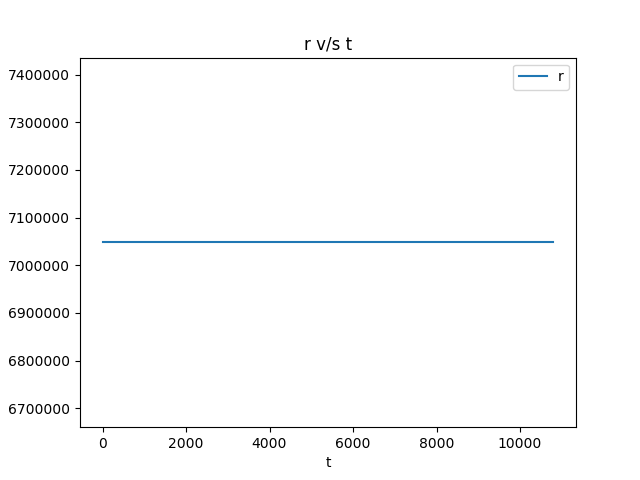
\includegraphics[width = 0.8\textwidth]{r_arr0.png}
 \caption{Variation of satellite distace from centre of earth with time}
\end{figure}

\begin{figure}[H]
 \centering
 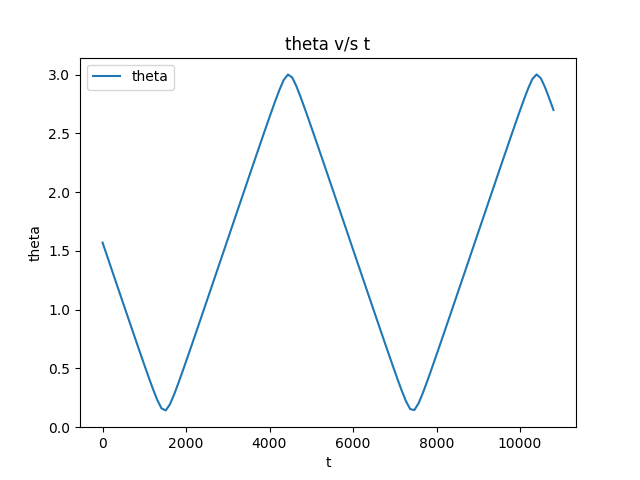
\includegraphics[width = 0.8\textwidth]{t_arr0.png}
 \caption{Variation of co-latitude from centre of earth with time}
\end{figure}

\begin{figure}[H]
 \centering
 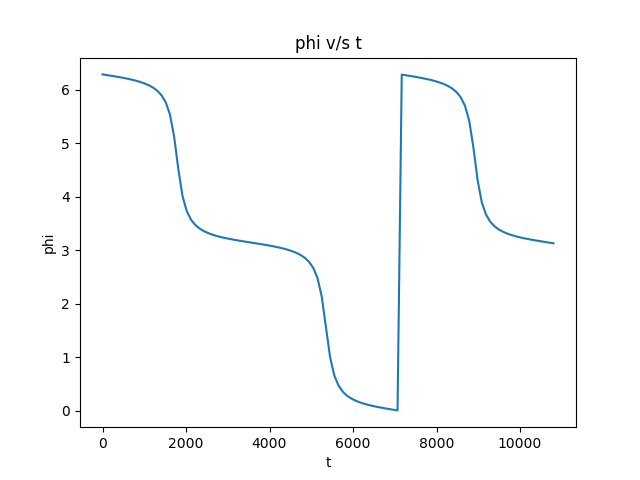
\includegraphics[width = 0.8\textwidth]{phi_arr0.png}
 \caption{Variation of phi from centre of earth with time}
\end{figure}


$V_r$ graph is weird. Yet to be explained

Initially it was felt that these numerical errors could be reduced by using $v_{\theta}, v_{\phi}$ instead of $\dot{\theta}, 
\dot{\phi}$ since $v_{\theta}, v_{\phi}$ are of the same order as $v_r$. But the value of $r$ kept on increasing on doing so.
Behavior yet to be explained


\section{Setting B accordng to IGRF model:}
\emph{May 5, 2017} \\

Simulation for 2 days. ( Run time \~8 hrs)

\subsection{Assumptions:}
\begin{itemize}
 \item No orbital perturbations due to oblateness of the earth
 \item Current in the tether equal to the current induced in radial direction
 \item Tether always pointing downwards.
\end{itemize}

\subsection{Results:}
\begin{figure}[H]
 \centering
 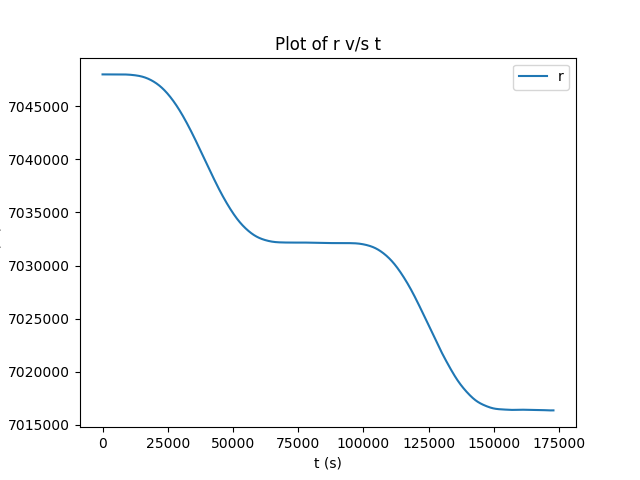
\includegraphics[width = 0.8\textwidth]{2dayr_.png}
 \caption{Variation of satellite distace from centre of earth with time}
\end{figure}

Initially the satellite orbit is very close to magnetic axis. So derobitting rate is small. After about half a day, magnetic 
makes largest angle with orbit, thus deorbiting rate is highest and starts decreasing again. Smae behaviour repeated for 
the next day. An average of about 15km/day.

\begin{figure}[H]
 \centering
 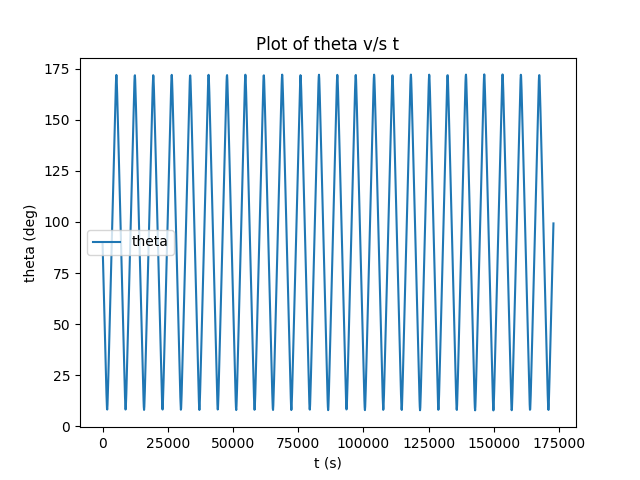
\includegraphics[width = 0.8\textwidth]{2daythet_.png}
 \caption{Variation of co-latitude with time}
\end{figure}

\begin{figure}[H]
 \centering
 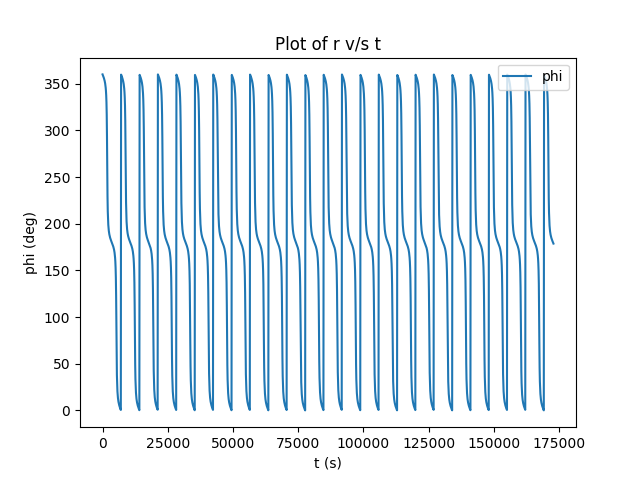
\includegraphics[width = 0.8\textwidth]{2dayp_.png}
 \caption{Variation of phi with time}
\end{figure}

Intuition says that the orbit should precess with time. But no such thing observed. (wondering why)

\begin{figure}[H]
 \centering
 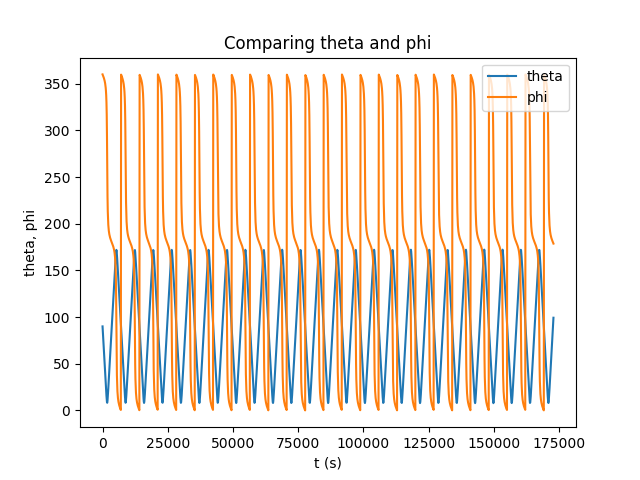
\includegraphics[width = 0.8\textwidth]{2dayt_p_.png}
 \caption{Variation of theta and phi}
\end{figure}


\section{Things to do next:}
\begin{itemize}
 \item Include perturbations due to earth being an ellipsoid
 \item Better model of current in Tether - Tanya and Anuj required
 \item Debugging for r0 and thetherv
 \item Keep wondering why no precession is observed or is it observed
\end{itemize}


\end{document}

